\documentclass{article}

\PassOptionsToPackage{numbers,compress}{natbib}
\usepackage[final]{neurips_2023}

\usepackage[utf8]{inputenc}
\usepackage[T1]{fontenc}
\usepackage{hyperref}
\usepackage{url}
\usepackage{amsmath}
\usepackage{amsfonts}
\usepackage{graphicx}
\usepackage{nicefrac}
\usepackage{microtype}
\usepackage{xcolor}

% The [final] option prints a NeurIPS conference notice in the footer.
% This is a course report, so the footer names the course instead.
% Margins, fonts and spacing are left exactly as the style file sets them.
\makeatletter
\renewcommand{\@noticestring}{COMP 560 Final Project, Fall 2026.}
\makeatother

\title{Finding the Root Cause of Cascading Failures\\with a Bayesian Network}

\author{%
  Dipendra Kandel \\
  PID: TODO \\
  \And
  Team Member 2 \\
  PID: TODO \\
  \And
  Team Member 3 \\
  PID: TODO \\
  \And
  Team Member 4 \\
  PID: TODO \\
  \AND
  Department of Computer Science, University of North Carolina at Chapel Hill
}

\begin{document}

\maketitle

\begin{abstract}
When one service in a large software system fails, the services that depend on
it often fail too, and monitoring fires a burst of alarms, some of them false.
We treat finding the original failure as diagnosis in a Bayesian network with a
hidden root cause, noisy-OR failure propagation along a dependency graph, and
noisy alarms. On simulated incidents we compare exact inference, likelihood
weighting, and two heuristics an engineer might use. Bayesian inference names
the right root cause more often than the heuristics at every noise level we
tried (0.74 vs.\ 0.65 top-1 accuracy at our default setting), and the gap
nearly triples as false alarms become common. Likelihood weighting matches
exact inference in accuracy and stays fast as the graph grows, while
enumeration becomes too slow at 18 services. Its estimates do degrade on
incidents with many alarms, where a few samples carry almost all the weight.
\end{abstract}

\section{Introduction}

Modern applications are built from many small services that call one another.
If a database goes down, every service that reads from it starts returning
errors, and so does everything downstream of those. The on-call engineer sees a
wall of alarms and has to work out which one points at the cause. Monitoring is
noisy, so a healthy service sometimes raises an alarm (a false positive) and a
broken one sometimes stays quiet (a false negative). Failures also do not
always spread, so the set of broken services changes from one incident to the
next.

A common rule of thumb is to look at the alarm furthest upstream. That works
when alarms are clean, but one false alarm upstream of the real fault sends the
engineer the wrong way. A probabilistic model can instead weigh how likely the
whole alarm pattern is under each possible cause. We ask (1) whether posterior
inference in a Bayesian network finds the root cause more often than simple
heuristics, and how that depends on alarm noise, and (2) how exact and
sampling-based inference compare in accuracy and run time as the graph and the
noise grow.

We simulate thousands of incidents on random dependency graphs and score each
method by whether it ranks the true root cause first (top-1) or in its first
three guesses (top-3). Nothing is learned. All probabilities are set by hand
and all data comes from the model, so the true cause is always known. Our code
and an interactive demo reproduce every number in this
paper.\footnote{\url{https://github.com/dipendrak/incident-detective}}

\section{Related work}

The QMR-DT network for medical diagnosis \citep{shwe1991qmr} links hundreds of
diseases to thousands of findings with noisy-OR factors
\citep{pearl1988probabilistic}. Exact inference in it is intractable, which led
to approximations such as variational methods \citep{jaakkola1999qmr}. Our
model has the same shape at a much smaller scale. Fault localization in
computer networks has its own long literature \citep{steinder2004survey}.
Sherlock \citep{bahl2007sherlock} infers service dependencies and searches for
the most likely set of failed components, and NetMedic
\citep{kandula2009netmedic} ranks culprits using component history. Those
systems work with real data. We aim for a controlled comparison of textbook
inference methods against heuristics, with known ground truth.

Exact inference in Bayesian networks is NP-hard \citep{cooper1990complexity},
and so is approximating it to a fixed relative error
\citep{dagum1993approximating}. Variable elimination \citep{zhang1994simple}
and junction trees \citep{lauritzen1988local} use graph structure to beat
brute-force enumeration. Likelihood weighting
\citep{fung1990weighing,shachter1990simulation} is the simplest importance
sampler for these networks and is known to struggle when the evidence is
unlikely under the prior, which motivated adaptive proposals such as AIS-BN
\citep{cheng2000aisbn} and Gibbs sampling \citep{pearl1987evidential}. We
follow \citet{russell2020aima} for both inference algorithms.

\section{Model and methods}

\paragraph{Dependency graph.}
A system has $N$ services. An edge $j \to i$ means service $i$ depends on $j$,
so a failure can flow from $j$ to $i$. In our random graphs, service $i$ draws
a number of parents uniformly from $\{0,\dots,\min(3,i)\}$ and picks them
uniformly among services $0,\dots,i-1$, so the numbering is a topological
order.

\paragraph{Bayesian network.}
The root cause $R$ is uniform over the $N$ services, with exactly one fault
per incident. Each service has a hidden failure state $F_i$. The root always
fails, and any other service fails with the noisy-OR probability
\begin{equation}
  P(F_i = 1 \mid \text{parents}) = 1 - (1-\lambda)(1-p)^{k_i},
\end{equation}
where $k_i$ counts failed parents, $p$ is the chance that one failed parent
brings $i$ down, and $\lambda$ is a small leak. Each service also has an
observed alarm $A_i$ with false-positive rate
$\alpha = P(A_i = 1 \mid F_i = 0)$ and false-negative rate
$\beta = P(A_i = 0 \mid F_i = 1)$. By default $N = 12$, $p = 0.7$,
$\lambda = 0.01$, $\alpha = 0.05$ and $\beta = 0.1$. Every method takes the
alarm vector $\mathbf{a}$ and returns a ranking of suspects.

\paragraph{Exact inference.}
With the uniform prior on $R$ cancelling,
\begin{equation}
  P(R = r \mid \mathbf{a}) \;\propto\; \sum_{\mathbf{f}\,:\,f_r = 1}\;
  \prod_{i \neq r} P(f_i \mid \mathbf{f}_{\text{pa}(i)})\;
  \prod_{i} P(a_i \mid f_i).
\end{equation}
We list all $2^N$ failure vectors as rows of a matrix and evaluate the sum in
log space with NumPy. We kept this brute force on purpose so that its $2^N$
cost shows up clearly.

\paragraph{Likelihood weighting.}
Each sample draws $R$ uniformly, simulates the cascade forward from the prior,
and gets weight $w = \prod_i P(a_i \mid f_i)$. The estimate of
$P(R = r \mid \mathbf{a})$ is the share of total weight held by samples with
root $r$. Cost is linear in $N$ and in the number of samples $S$. We also
report the effective sample size $\text{ESS} = (\sum w)^2 / \sum w^2$
\citep{kong1992note}, the number of equally weighted samples the uneven
weights are worth.

\paragraph{Baselines.}
\emph{Most upstream alarm} ranks alarmed services in topological order, then
silent ones. \emph{Most alarmed descendants} ranks alarmed services by how many
of their downstream services also alarm, since a true root should explain many
alarms below it. \emph{Random} gives chance level.

\section{Experiments}

Each incident picks a root cause, simulates the cascade and draws alarms. Only
the alarms reach the methods. Incident $k$ uses a fresh random graph with seed
$560 + k$, so results average over graph shapes as well as incidents. We report
95\% Wilson intervals \citep{wilson1927probable}. Seeds are fixed, so a rerun
gives the same numbers apart from run times.

\begin{figure}[t]
  \centering
  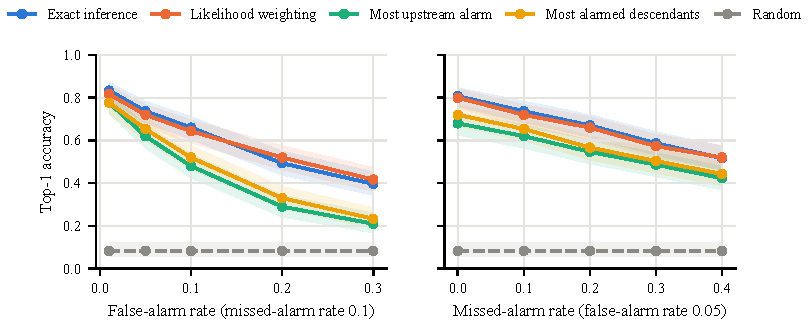
\includegraphics[width=\linewidth]{figures/accuracy.pdf}
  \caption{Top-1 accuracy as alarms get noisier ($N = 12$, 300 incidents per
  point, bands are 95\% intervals). Left: more false alarms. Right: more missed
  alarms.}
  \label{fig:accuracy}
\end{figure}

\subsection{Accuracy against the heuristics}

We ran 300 incidents per noise setting, with 5,000 samples for likelihood
weighting. At the default setting, exact inference ranks the true root first
in 0.74 of incidents (95\% CI 0.68 to 0.78) and likelihood weighting in 0.72.
Most alarmed descendants reaches 0.65, most upstream alarm 0.62, and random
guessing 0.08. Top-3 accuracy is 0.93 for exact inference and 0.89 for both
heuristics.

Figure~\ref{fig:accuracy} shows the effect of noise. With rare false alarms
($\alpha = 0.01$) the methods are close, at 0.83 for exact inference and 0.78
for the heuristics. As $\alpha$ rises the heuristics fall much faster, and at
$\alpha = 0.3$ exact inference gets 0.40 against 0.23 for the best heuristic,
so the top-1 gap grows from 0.06 to 0.16. Both heuristics treat every alarm as
true, and a single false alarm upstream of the real fault is enough to fool
most-upstream. The posterior asks how likely the whole pattern is under each
candidate, and under the model an isolated alarm with no failed neighbors is
cheap to explain as noise. Missed alarms hurt all methods about equally, and
the gap stays between 0.07 and 0.10 across that sweep. Exact inference and
likelihood weighting are within sampling noise of each other at every point.

\begin{figure}[t]
  \centering
  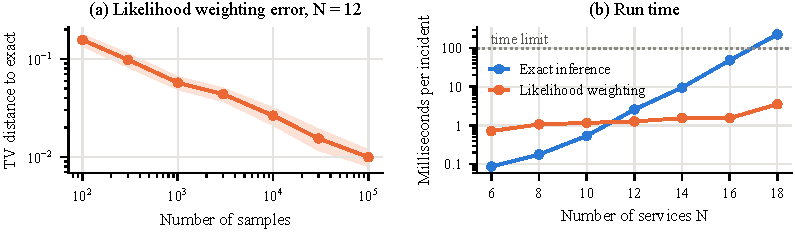
\includegraphics[width=\linewidth]{figures/cost.pdf}
  \caption{(a) Total variation (TV) distance from the likelihood weighting
  estimate to the exact posterior ($N = 12$, 200 incidents). (b) Mean run time
  per incident on a laptop (100 incidents per size). Exact inference was
  stopped at $N = 18$ after exceeding 0.1\,s per incident.}
  \label{fig:cost}
\end{figure}

\subsection{Sampling error and run time}

On 200 incidents, the total variation distance between likelihood weighting
and the exact posterior falls from 0.156 with 100 samples to 0.057 with 1,000
and 0.010 with 100,000 (Figure~\ref{fig:cost}a). The log-log slope is about
$-0.4$, a little slower than the $1/\sqrt{S}$ rate of plain Monte Carlo. The
ESS is only 5\% to 10\% of the raw sample count (65 at $S = 1{,}000$, 5,446 at
$S = 100{,}000$) because most forward samples look nothing like the observed
alarms. The top suspect matches the exact one in 0.91 of incidents at 1,000
samples and levels off around 0.93 to 0.94. Of the 13 incidents that still
disagree at 100,000 samples, 12 have their top two exact suspects within 0.005
of each other, usually two services the alarms cannot tell apart. The last has
a gap of 0.026.

Exact inference takes 0.1\,ms per incident at $N = 6$ and 2.6\,ms at $N = 12$,
and every two extra services then multiply its time by about four to five
(Figure~\ref{fig:cost}b). It needs 48\,ms at $N = 16$, and at $N = 18$ its
first incidents averaged 225\,ms, so we stopped it at our 0.1\,s limit.
Likelihood weighting with 5,000 samples grows from 0.7\,ms to 3.5\,ms over the
same range and becomes the faster method between $N = 10$ and $N = 12$.
Wherever exact inference finished, the two had the same top-1 accuracy within
noise (0.64 and 0.64 at $N = 16$).

\begin{figure}[t]
  \centering
  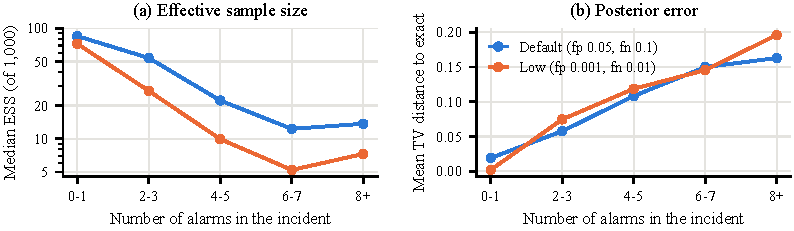
\includegraphics[width=\linewidth]{figures/failure.pdf}
  \caption{Likelihood weighting with 1,000 samples, grouped by number of
  alarms ($N = 12$, 2,000 incidents per noise setting). (a) Median effective
  sample size. (b) Mean TV distance to the exact posterior.}
  \label{fig:failure}
\end{figure}

\subsection{When likelihood weighting struggles}

Likelihood weighting ignores the alarms until it computes the weights, and
every service where a sample disagrees with the alarms costs a factor of
$\alpha$ or $\beta$. With many alarms, few forward samples come close to the
observed pattern. We grouped 2,000 incidents by their number of alarms, at
default noise and at low noise ($\alpha = 0.001$, $\beta = 0.01$), using 1,000
samples (Figure~\ref{fig:failure}). At low noise the median ESS falls from 72
with zero or one alarm to between 5 and 7 with six or more. Lower noise makes
the drop steeper because the penalty factors are smaller. The error grows in
both settings, from 0.002 to 0.20 at low noise and from 0.02 to 0.16 at default
noise, so the number of alarms matters more than the noise level. Top-1
accuracy suffers less, losing at most 0.04 against exact inference. Still, the
probabilities reported for large incidents are much less accurate, and those
are the incidents where an engineer most needs a clear answer. A low ESS is
cheap to compute and signals that more samples, or a proposal that looks at the
alarms \citep{cheng2000aisbn}, are needed.

\section{Limitations}

All data is simulated from the same model used for inference, and the Bayesian
methods are given the true $p$, $\lambda$, $\alpha$ and $\beta$. In practice
these would be estimated, and wrong values could hurt the Bayesian methods
while the heuristics would not notice. We assume one root cause per incident.
Our graphs are small random DAGs without the hubs, cycles and hundreds of
services of real systems, and our alarms are independent given the failures,
while real alarms are often correlated. Finally, our exact method is
brute-force enumeration. Variable elimination would push the size limit
further on sparse graphs, so the crossover in Figure~\ref{fig:cost}b describes
our implementation, not exact inference in general.

\section{Conclusion}

In this simulated setting, a small Bayesian network finds the root cause of a
cascading failure more often than common rules of thumb, and its advantage
grows as alarms become less trustworthy. Likelihood weighting matches exact
inference in accuracy at a fraction of the cost on larger graphs, but its
estimates degrade on incidents with many alarms, which shows up as a low
effective sample size. Natural next steps are learning the noise rates from
incident history, allowing several root causes, and testing on real service
topologies.

\bibliographystyle{plainnat}
\bibliography{references}

\end{document}
